\section{Конструкторская часть}

В этом разделе будут представлено описание используемых типов данных, а также схемы алгоритмов вычисления расстояния Левенштейна и Дамерау~---~Левенштейна.

\subsection{Нерекурсивный алгоритм нахождения расстояния Левенштейна}

Схема нерекурсивного алгоритма нахождения расстояния Левенштейна представлена на рисунке \ref{img:lev}.

\begin{figure}[h]
	\centering
	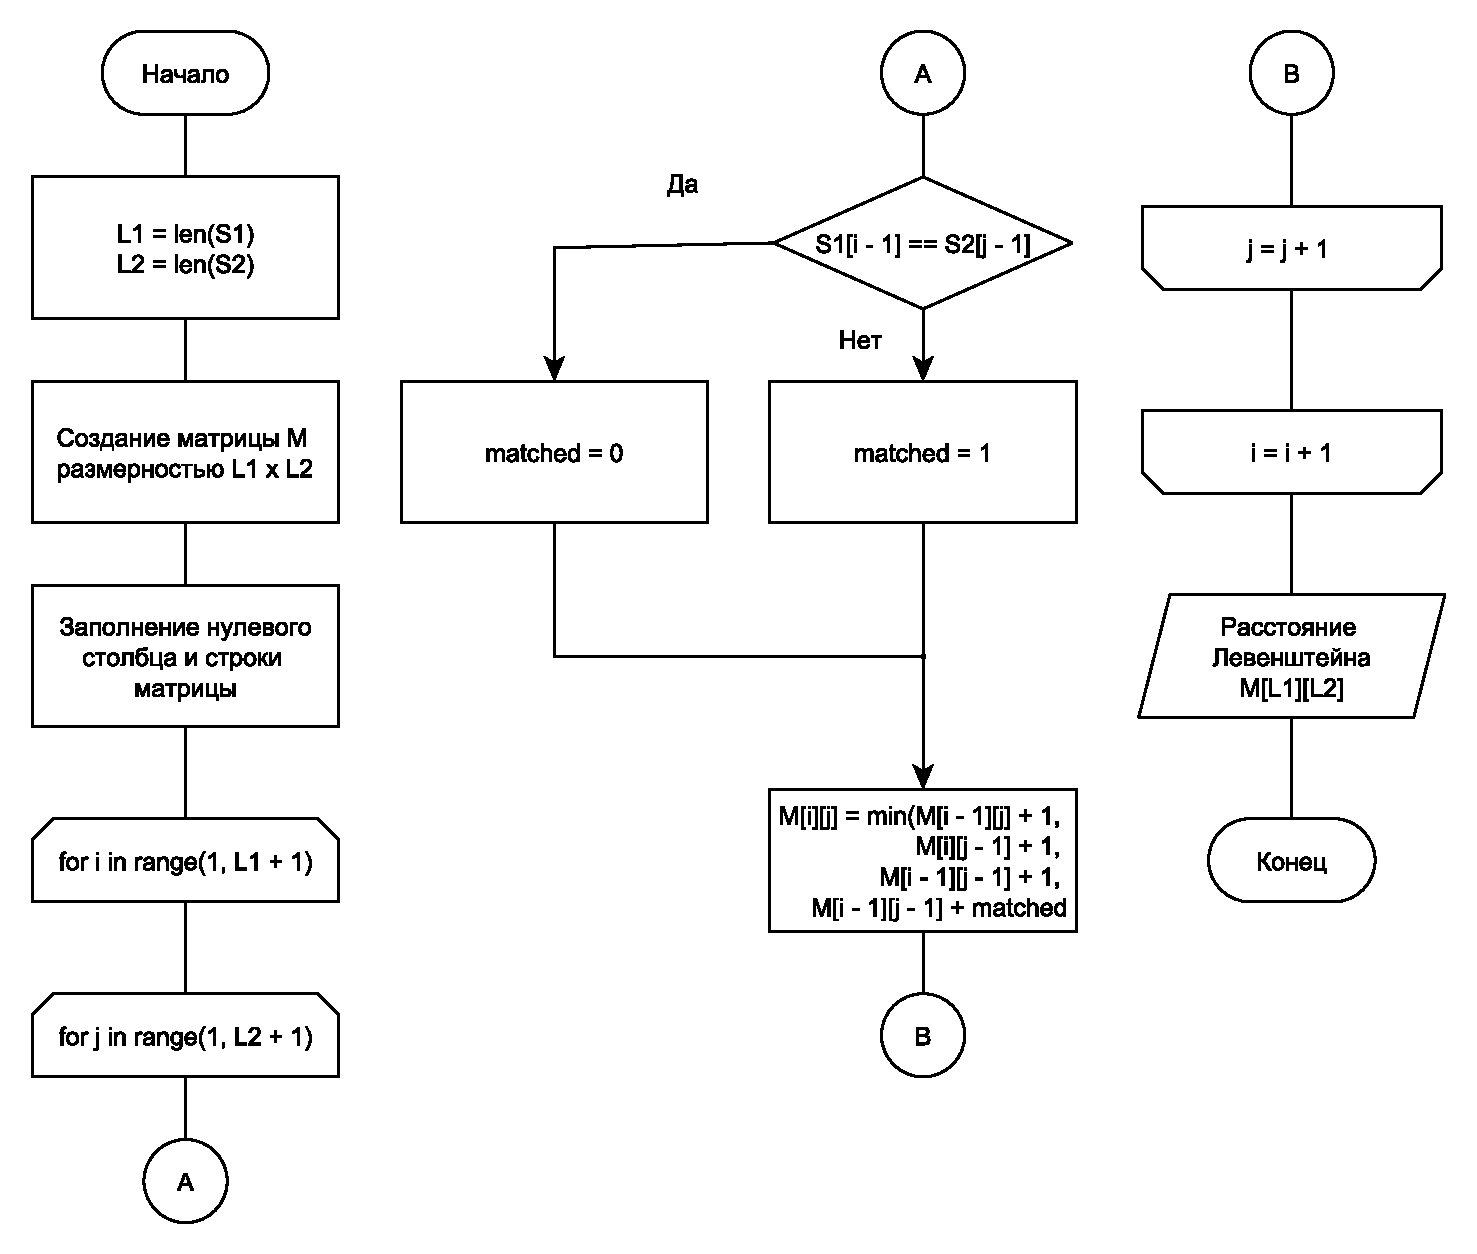
\includegraphics[scale=0.6]{images/lev.pdf}
	\caption{Схема нерекурсивного алгоритма нахождения расстояния Левенштейна}
	\label{img:lev}
\end{figure}

\newpage

\subsection{Нерекурсивный алгоритм нахождения расстояния Дамерау~---~Левенштейна}

Схема нерекурсивного алгоритма нахождения расстояния Дамерау~---~Левенштейна представлена на рисунке \ref{img:dlev}.

\begin{figure}[h]
	\centering
	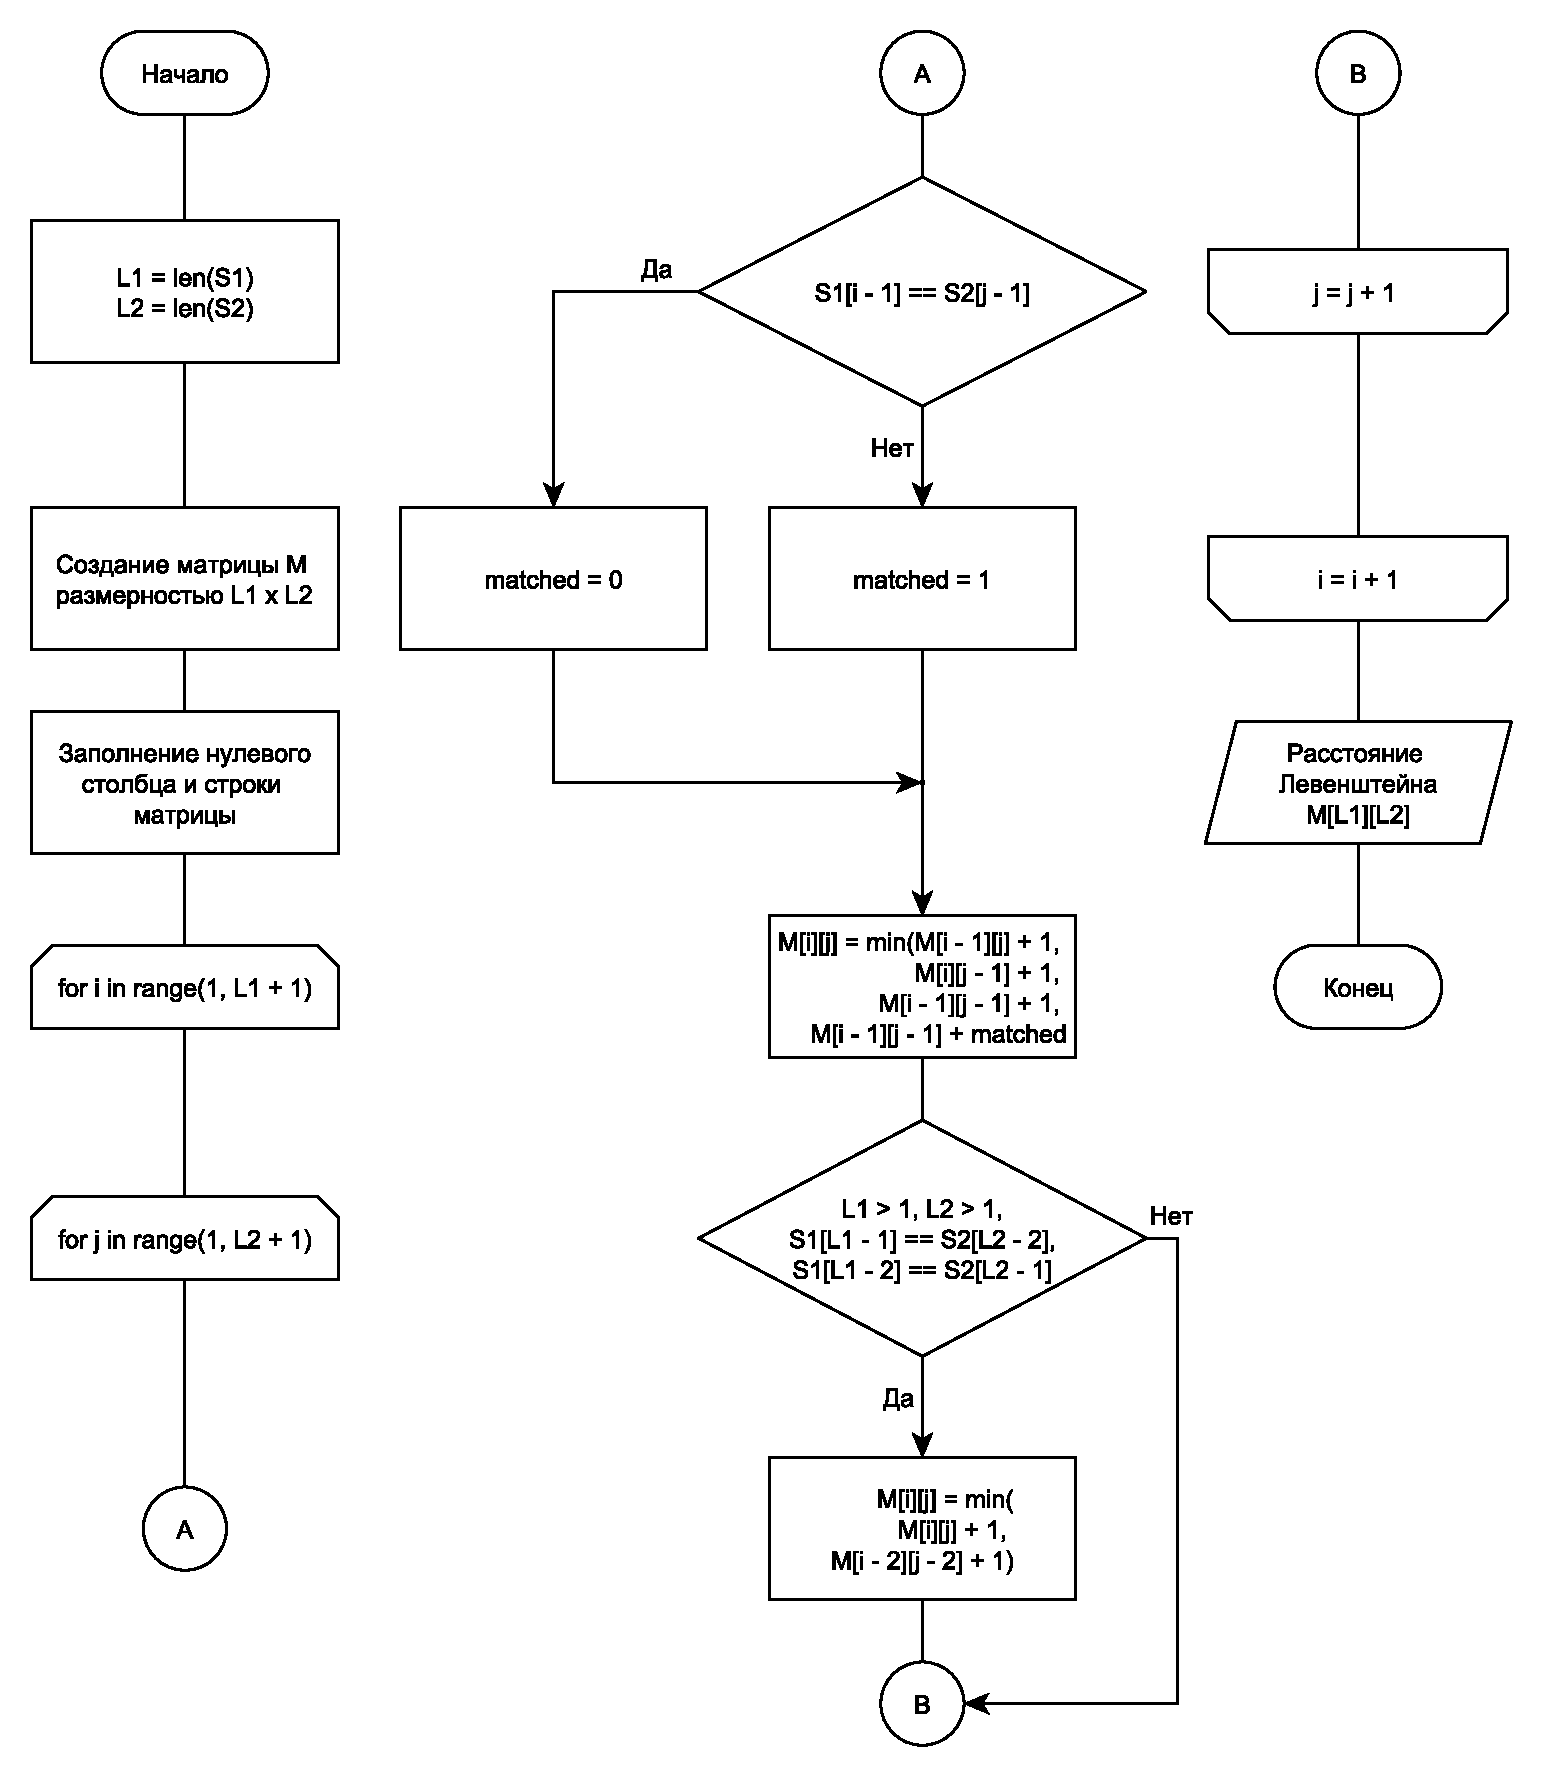
\includegraphics[scale=0.6]{images/dlev.pdf}
	\caption{Схема нерекурсивного алгоритма нахождения расстояния Дамерау~---~Левенштейна}
	\label{img:dlev}
\end{figure}


\subsection{Рекурсивный алгоритм нахождения расстояния Дамерау~---~Левенштейна}

Схема рекурсивного алгоритма нахождения расстояния Дамерау~---~Левенштейна представлена на рисунке \ref{img:dlev_req}.

\begin{figure}[h]
	\centering
	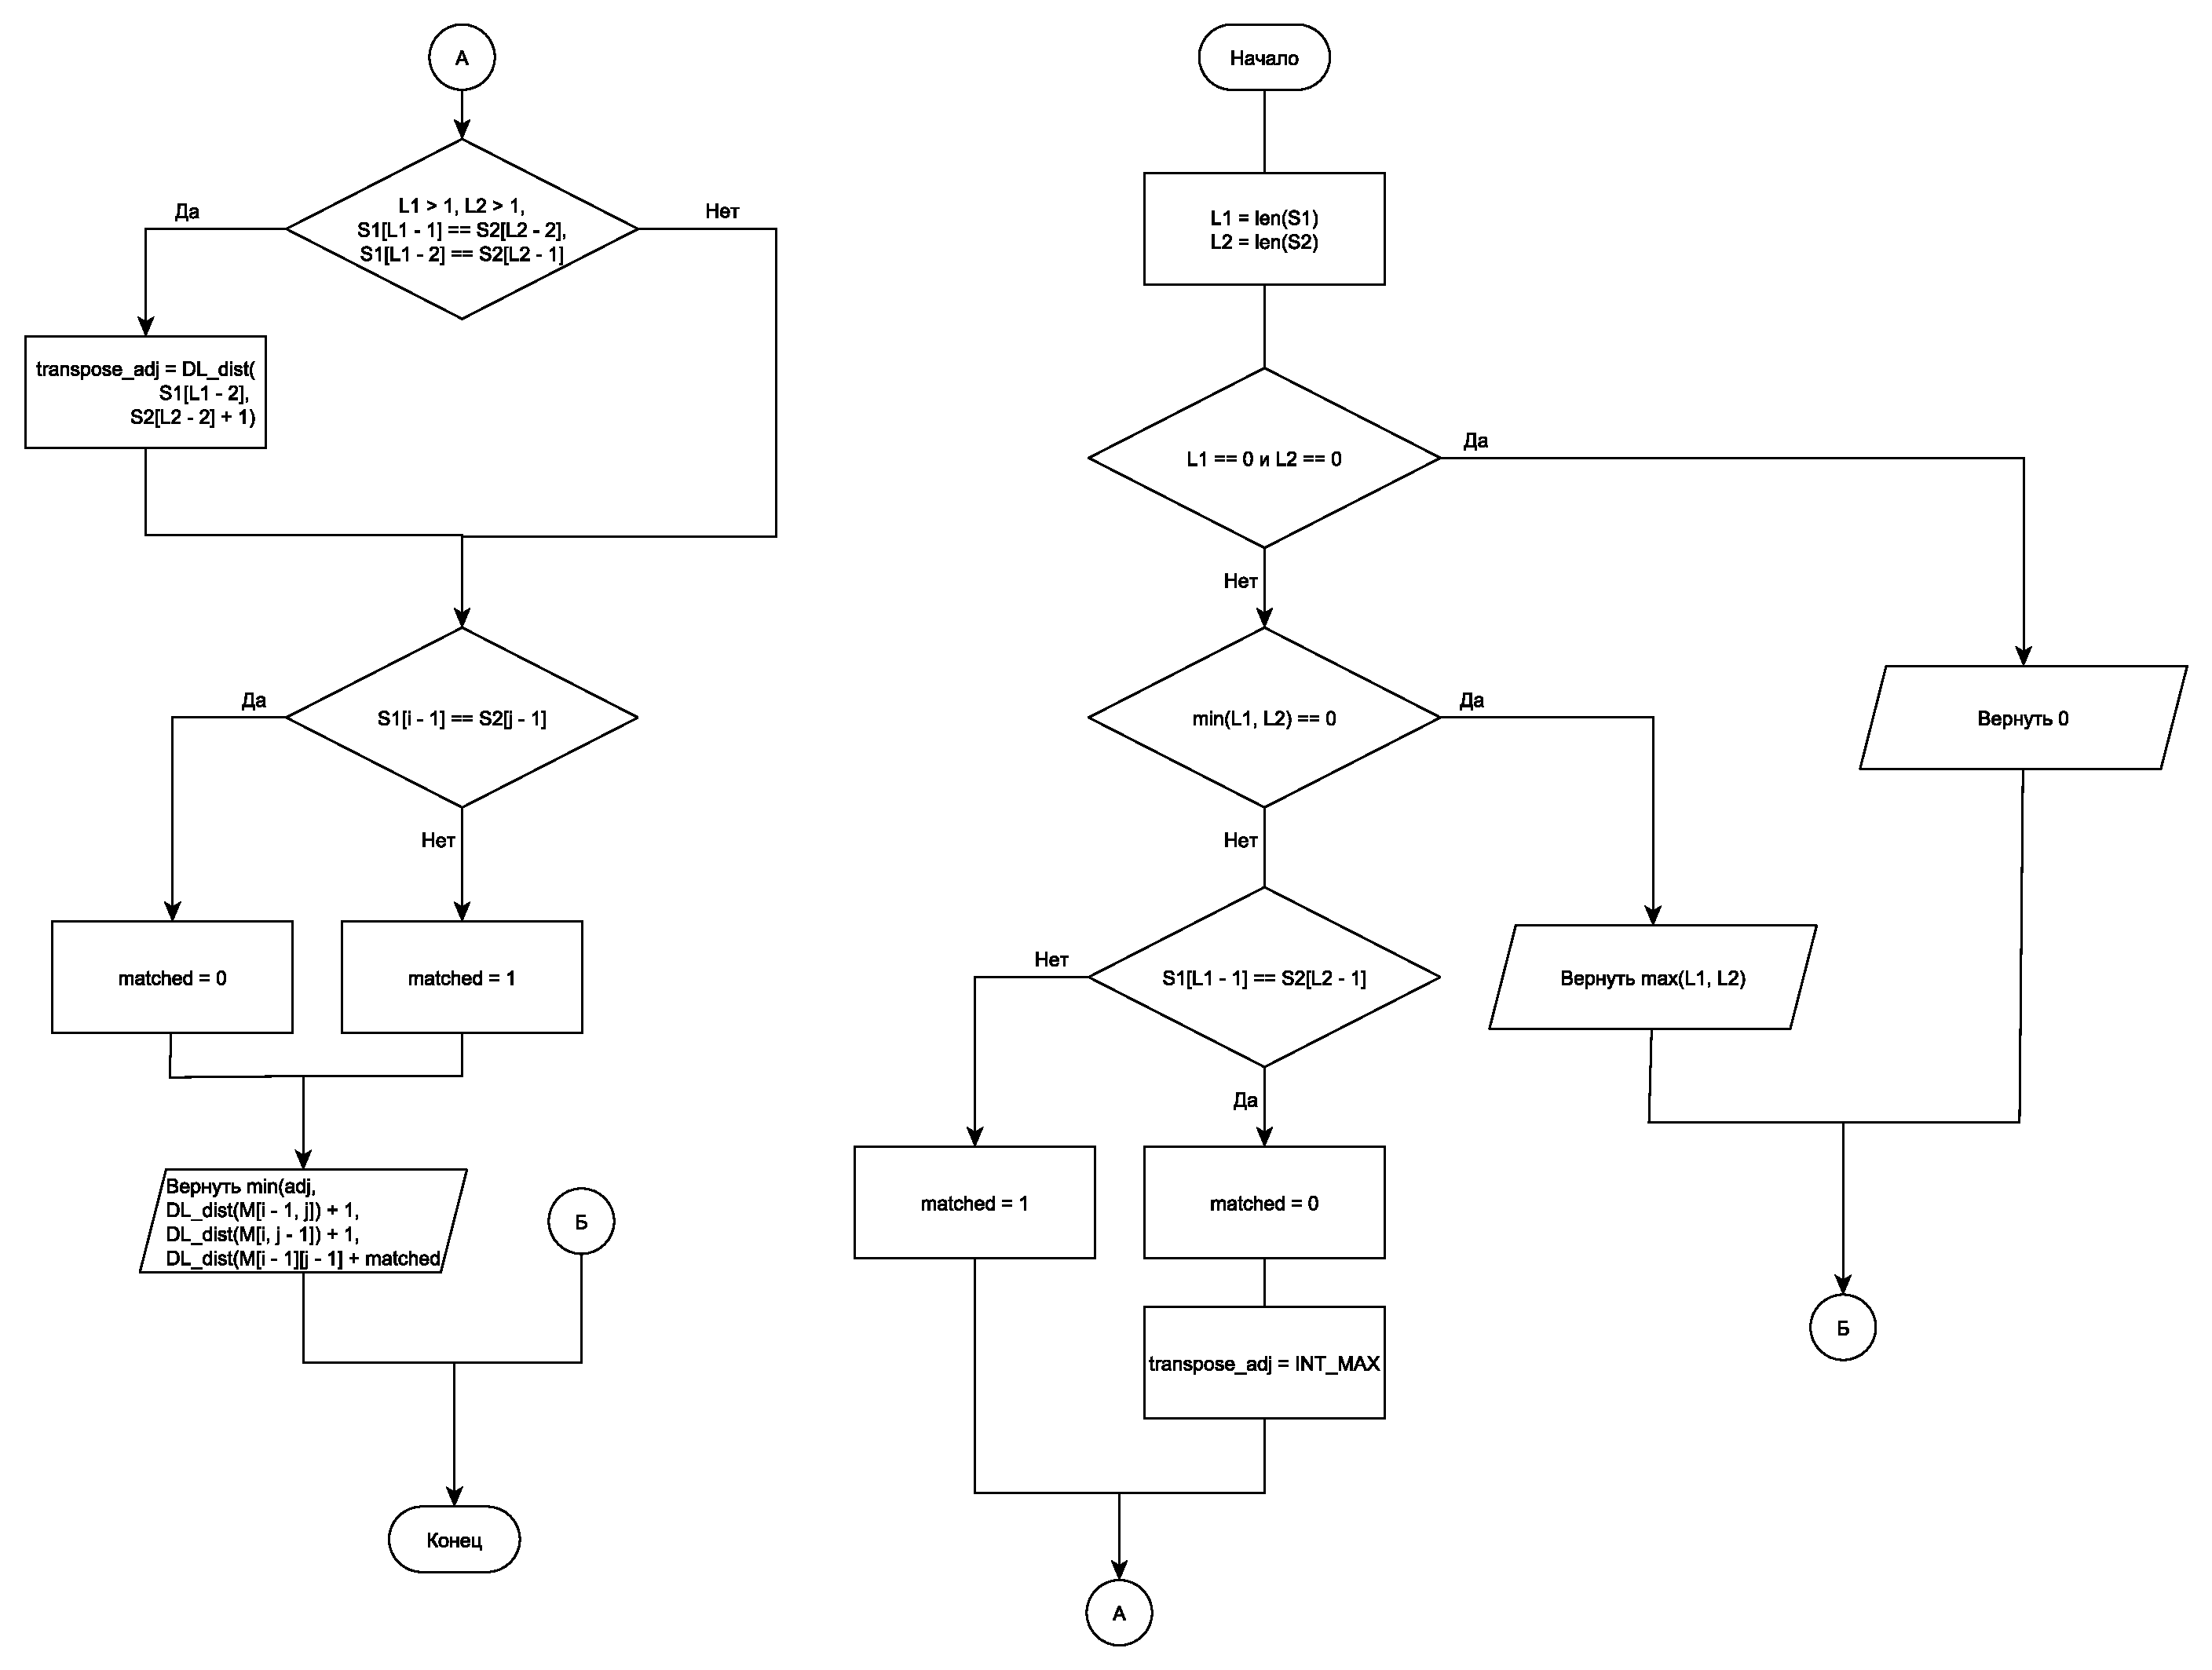
\includegraphics[scale=0.35]{images/dlev_req.pdf}
	\caption{Схема рекурсивного алгоритма нахождения расстояния Дамерау~---~Левенштейна}
	\label{img:dlev_req}
\end{figure}

\newpage

\subsection{Рекурсивный алгоритм нахождения расстояния Дамерау~---~Левенштейна с кэшем}

Схема рекурсивного алгоритма нахождения расстояния Дамерау~---~Левенштейна с кэшем представлена на рисунке \ref{img:dlev_req_cache}.

\begin{figure}[h]
	\centering
	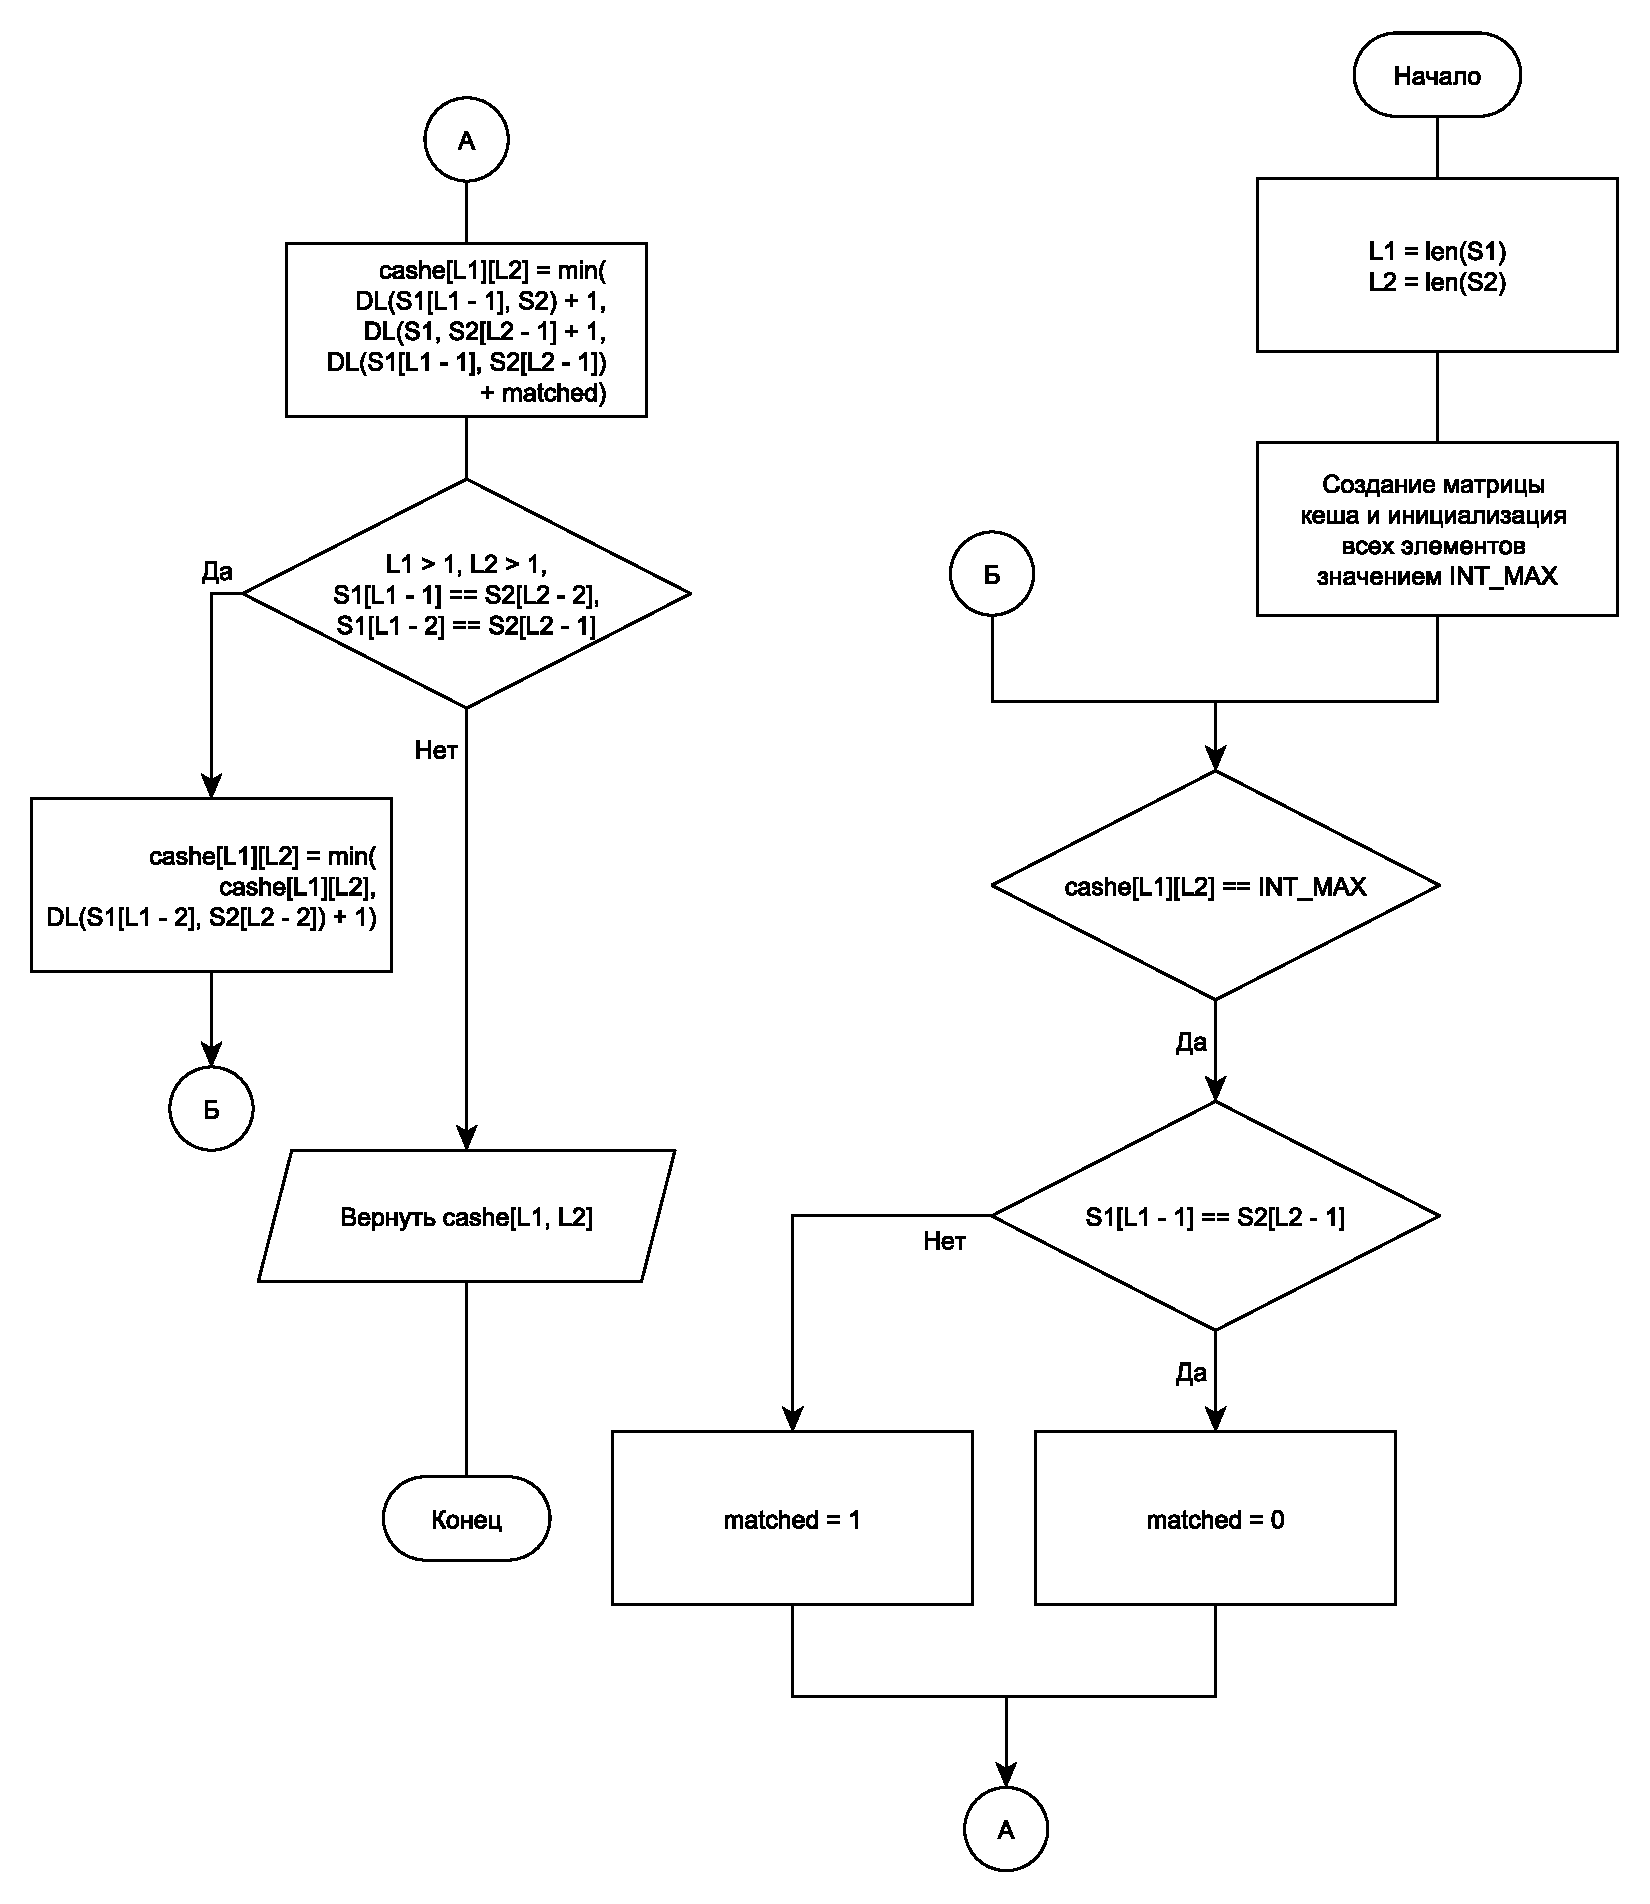
\includegraphics[scale=0.55]{images/dlev_req_cache.pdf}
	\caption{Схема рекурсивного алгоритма нахождения расстояния Дамерау~---~Левенштейна с кэшем}
	\label{img:dlev_req_cache}
\end{figure}

